%Optics Homework_2
\documentclass[10pt,a4paper]{article}
\usepackage[UTF8]{ctex}
\usepackage{bm}
\usepackage{amsmath}
\usepackage{extarrows}
\usepackage{amsthm}
\usepackage{amssymb}
\usepackage{graphicx}
\usepackage{multirow}
\title{光学作业\#2}
\author{陈稼霖 \and 45875852}
\date{2018.10.10}
\theoremstyle{remark}
\newtheorem{defi}{Definition}
\newtheorem{cdefi}{\bf 定义}
\begin{document}
\maketitle
\section*{2-2}证:
如图2-6,
\begin{align*}
&\because\frac{\overline{CQ}}{\overline{CM}} = \frac{\frac{n'}{n}r}{r} = \frac{\overline{CM}}{\overline{CQ'}} = \frac{r}{\frac{n}{n'}r} = \frac{n'}{n}\\
&\therefore\triangle CQM \backsim \triangle CMQ'\\
&\therefore u' = \angle CQ'M = \angle CMQ
\end{align*}
故根据正弦定理
\begin{align*}
\text{原式左边} = \frac{\sin u}{\sin u'} = \frac{\overline{CM}}{\overline{CQ}} = \frac{r}{\frac{n'}{n}r} = \frac{n}{n'}
\end{align*}
又
\[
\text{原式右边} = \frac{\overline{AQ'}}{\overline{QA}} = \frac{r + \frac{n}{n'}r}{r + \frac{n'}{n}r} = \frac{n}{n'}
\]
故
\[
\text{原式左边} = \text{原式右边}
\]
式(2-4)成立。
%\section*{2-4}解:
%设凹球面反射镜的曲率半径为$-R~(-R > 0)$,凹球面反射镜的物像距公式和横向放大率分别为
%\begin{align*}
%&\frac{1}{s'} + \frac{1}{s} = -\frac{2}{R}\\
%&V = -\frac{s'}{s} = -1\\
%&\Longrightarrow s = -R
%\end{align*}
%故物体放在凹球面反射镜球心处,可产生大小与物体相等的倒立实像。
\section*{2-5}解:
成放大两倍的实像,凹球面反射镜的物像距公式和横向放大率分别为
\begin{align*}
&\frac{1}{s'} + \frac{1}{s} = -\frac{2}{R} = -\frac{2}{-40cm}\\
&V = -\frac{s'}{s} = -2\\
&\Longrightarrow s = 30cm
\end{align*}
故要成放大两倍的实像,物体应放在凹面镜前距凹面镜顶点$30cm$的傍轴处。

成放大两倍的虚像,凹球面反射镜的物像距公式和横向放大率分别为
\begin{align*}
&\frac{1}{s'} + \frac{1}{s} = -\frac{2}{R} = -\frac{2}{-40cm}\\
&V = -\frac{s'}{s} = 2\\
&\Longrightarrow s = 10cm
\end{align*}
故要成放大两倍的实像,物体应放在凹面镜前距凹面镜顶点$30cm$的傍轴处。
\section*{2-6}解:
物距为$s = 10cm = 0.1m$,像距为$s' = 3m$,根据球面反射镜成像的物像距公式
\begin{align*}
&\frac{1}{s'} + \frac{1}{s} = -\frac{2}{r}\\
&r = -\frac{6}{31}m
\end{align*}
横向放大率为
\[
V = -\frac{s'}{s} = -30
\]
故镜形应该是凹的,半径应为$\frac{6}{31}m$,这时像放大了$30$倍(倒像)。
\section*{2-9}解:
题中所述情况下,凸球面折射镜的像方焦距恰好为球面半径的两倍
\begin{align*}
&f' = \frac{n'r}{n' - 1} = 2r\\
&\Longrightarrow n' = 2
\end{align*}
故此透明体的折射率应等于$2$。
\section*{2-11}解:
将平行玻璃板的前后表面视为曲率半径无穷大的两个折射面,该光学系统的物距为$s_1 =  -(t + 15cm)$,最终成像的像距为$15cm + 3cm$,第一次折射的物像距公式为
\[
\frac{1.5}{s'_1} + \frac{1}{s_1} = 0
\]
第一次折射的像距和第二次折射的物距之间的几何关系为
\[
s'_1 + s_2 = t
\]
第二次折射的物像距公式为
\[
\frac{1}{15cm + 3cm} + \frac{1.5}{s_2} = 0
\]
以上三式联立解得玻璃板的厚度
\[
t = 9cm
\]
\section*{2-13}解:
如书中图2-7,设$\Sigma$为折射球面,其半径为$r$,球心位于$C$,顶点为$A$,前后介质的折射率分别为$n$和$n'$,从轴上物点$Q$引一条入射光线与$\Sigma$相遇于$M$,折射后重新交于$Q'$,令
\[
\overline{QA} = s, \overline{AQ'} = s', \overline{QM} = p, \overline{MQ'} = p'
\]
$QM$、$MQ'$以及半径$CM$与光轴的夹角分别为$u$、$u'$和$\varphi$,入射角为$i$,折射角为$i'$。在几何上有余弦定理
\begin{align*}
&p = \sqrt{(s + r)^2 + r^2 - 2r(s + r)\cos\varphi}\\
&p' = \sqrt{(s' - r)^2 + r^2 + 2r(s' - r)\cos\varphi}
\end{align*}
从物点$Q$到像点$Q'$的光程为
\begin{align*}
(QP') &= np + n'p'\\
&\scalebox{0.95}{$= n\sqrt{(s + r)^2 + r^2 - 2r(s + r)\cos\varphi} + n'\sqrt{(s' - r)^2 + r^2 + 2r(s' - r)\cos\varphi}$}
\end{align*}
由于在傍轴情况下折射球面可近似成像,故从物点$Q$发出并到达像点$Q'$的任意一条光线都具有相同的光程,即光程$(QQ')$不随角度$\varphi$的改变而改变,即光程$(QQ')$对于角度$\varphi$的导数等于$0$
\begin{align*}
\frac{d(QP')}{d\varphi} &=  \scalebox{1}{$n\frac{r(s + r)\sin\varphi}{\sqrt{(s + r)^2 + r^2 - 2r(s + r)\cos\varphi}} - n'\frac{r(s' - n)\sin\varphi}{\sqrt{(s' - r)^2 + r^2 + 2r(s' - r)\cos\varphi}}$}\\
&= 0
\end{align*}
在傍轴条件下,$\varphi\to0$,故$\cos\varphi\to1$,代入上式得
\begin{align*}
&n\frac{r(s + r)\sin\varphi}{\sqrt{(s + r)^2 + r^2 - 2r(s + r)}} - n'\frac{r(s' - n)\sin\varphi}{\sqrt{(s' - r)^2 + r^2 + 2r(s' - r)}} = 0\\
\Longrightarrow&\scalebox{0.95}{$n(s + r)\sqrt{(s' - r)^2 + r^2 + 2r(s' - r)} = n'(s' - r)\sqrt{(s + r)^2 + r^2 - 2r(s + r)}$}\\
\Longrightarrow&n(s + r)s' = n'(s' - r)s\\
\Longrightarrow&\frac{n'}{s'} + \frac{n}{s} = \frac{n' - n}{r}
\end{align*}
即得证傍轴条件下球面折射成像公式。
\section*{1-17}解:
光穿过该空气透镜的过程中发生了四次折射。第一次折射(球面玻璃外表面处)的物像距公式为
\[
\frac{n_{glass}}{s'_1} + \frac{n_{water}}{s_1} = \frac{n_{glass} - n_{water}}{r}
\]
由于玻璃壁厚可忽略,故第一次折射的像距和第二次折射的物距之间存在几何关系
\[
s'_1 + s_2 = 0
\]
第二次折射(球面玻璃内表面处)的物像距公式为
\[
\frac{n_{air}}{s'_2} + \frac{n_{glass}}{s_2} = \frac{n_{air} - n_{glass}}{r}
\]
忽略空气层厚度,第二次折射的像距和第三次折射的物距之间存在几何关系
\[
s'_2 + s_3 = 0
\]
第三次折射(平面玻璃内表面处,可以视为曲率半径无穷大的折射球面)的物像距公式为
\[
\frac{n_{glass}}{s'_3} + \frac{n_{air}}{s_3} = 0
\]
由于玻璃壁厚可忽略,故第一次折射的像距和第二次折射的物距之间存在几何关系
\[
s'_3 + s_4 = 0
\]
第四次折射(平面玻璃外表面处,可以视为曲率半径无穷大的折射球面)的物像距公式为
\[
\frac{n_{water}}{s'_4} + \frac{n_{glass}}{s_4} = 0
\]
以上各式中球面玻璃折射半径$r = 20cm$,水和空气的折射率分别为$\frac{4}{3}$和$1$。
对于平行入射的入射光,$s_1$为无穷大,将其代入以上各式联立解得的$s'_4$即为像方焦距
\[
f' = s'_4 = -80cm
\]
对于平行出射的出射光,可以推知其在第二次折射后就达到平行,故$s'_2$为无穷大,将其代入以上各式联立解得的$s_1$即为物方焦距
\[
f = s_1 = -80cm
\]
(由于玻璃壁厚可忽略,也可以对该空气透镜直接用薄透镜焦距公式
\[\left\{\begin{array}{l}f = \frac{n}{\frac{n_L - n}{r_1} + \frac{n' - n_L}{r_2}} = \frac{n_{water}}{\frac{n_{air} - n_{water}}{r_1}}\\f' = \frac{n'}{\frac{n_L - n}{r_1} + \frac{n' - n_L}{r_2}} = \frac{n_{water}}{\frac{n_{air} - n_{water}}{r_1}}\end{array}\right.\]
直接得解。)

由于焦距为负值,故此透镜是发散的。
\section*{2-19}解:
如表(\ref{TableofProblem1-19})
\begin{table}[h]
\centering
\footnotesize
\begin{tabular}{| c | c | c | c | c | c | c | c | c |}
\hline
物距$s/cm$ & $-24$ & $-12$ & $-6.0$ & $0$ & $6.0$ & $12$ & $24$ & $36$ \\
\hline
像距$s'/cm$ & $-24$ & $\infty$ & $12$ & 0 & $-4$ & $-6$ & $-8$ & $-9$\\
\hline
横向放大率 & -1 & 不成像 & $2$ & 不成像 & $\frac{2}{3}$ & $\frac{1}{2}$ & $\frac{1}{3}$ & $\frac{1}{4}$\\
\hline
像的虚实 & 虚 & 不成像 & 实 & 不成像 & 虚 & 虚 & 虚 & 虚\\
\hline
像的正倒 & 倒 & 不成像 & 正 & 不成像 & 正 & 正 & 正 & 正\\
\hline
\end{tabular}
\caption{1-19题表}\label{TableofProblem1-19}
\end{table}

当物距为$-24cm$时,相应光路图如图(\ref{FigureofProblem2-19_1})
\begin{figure}
\centering
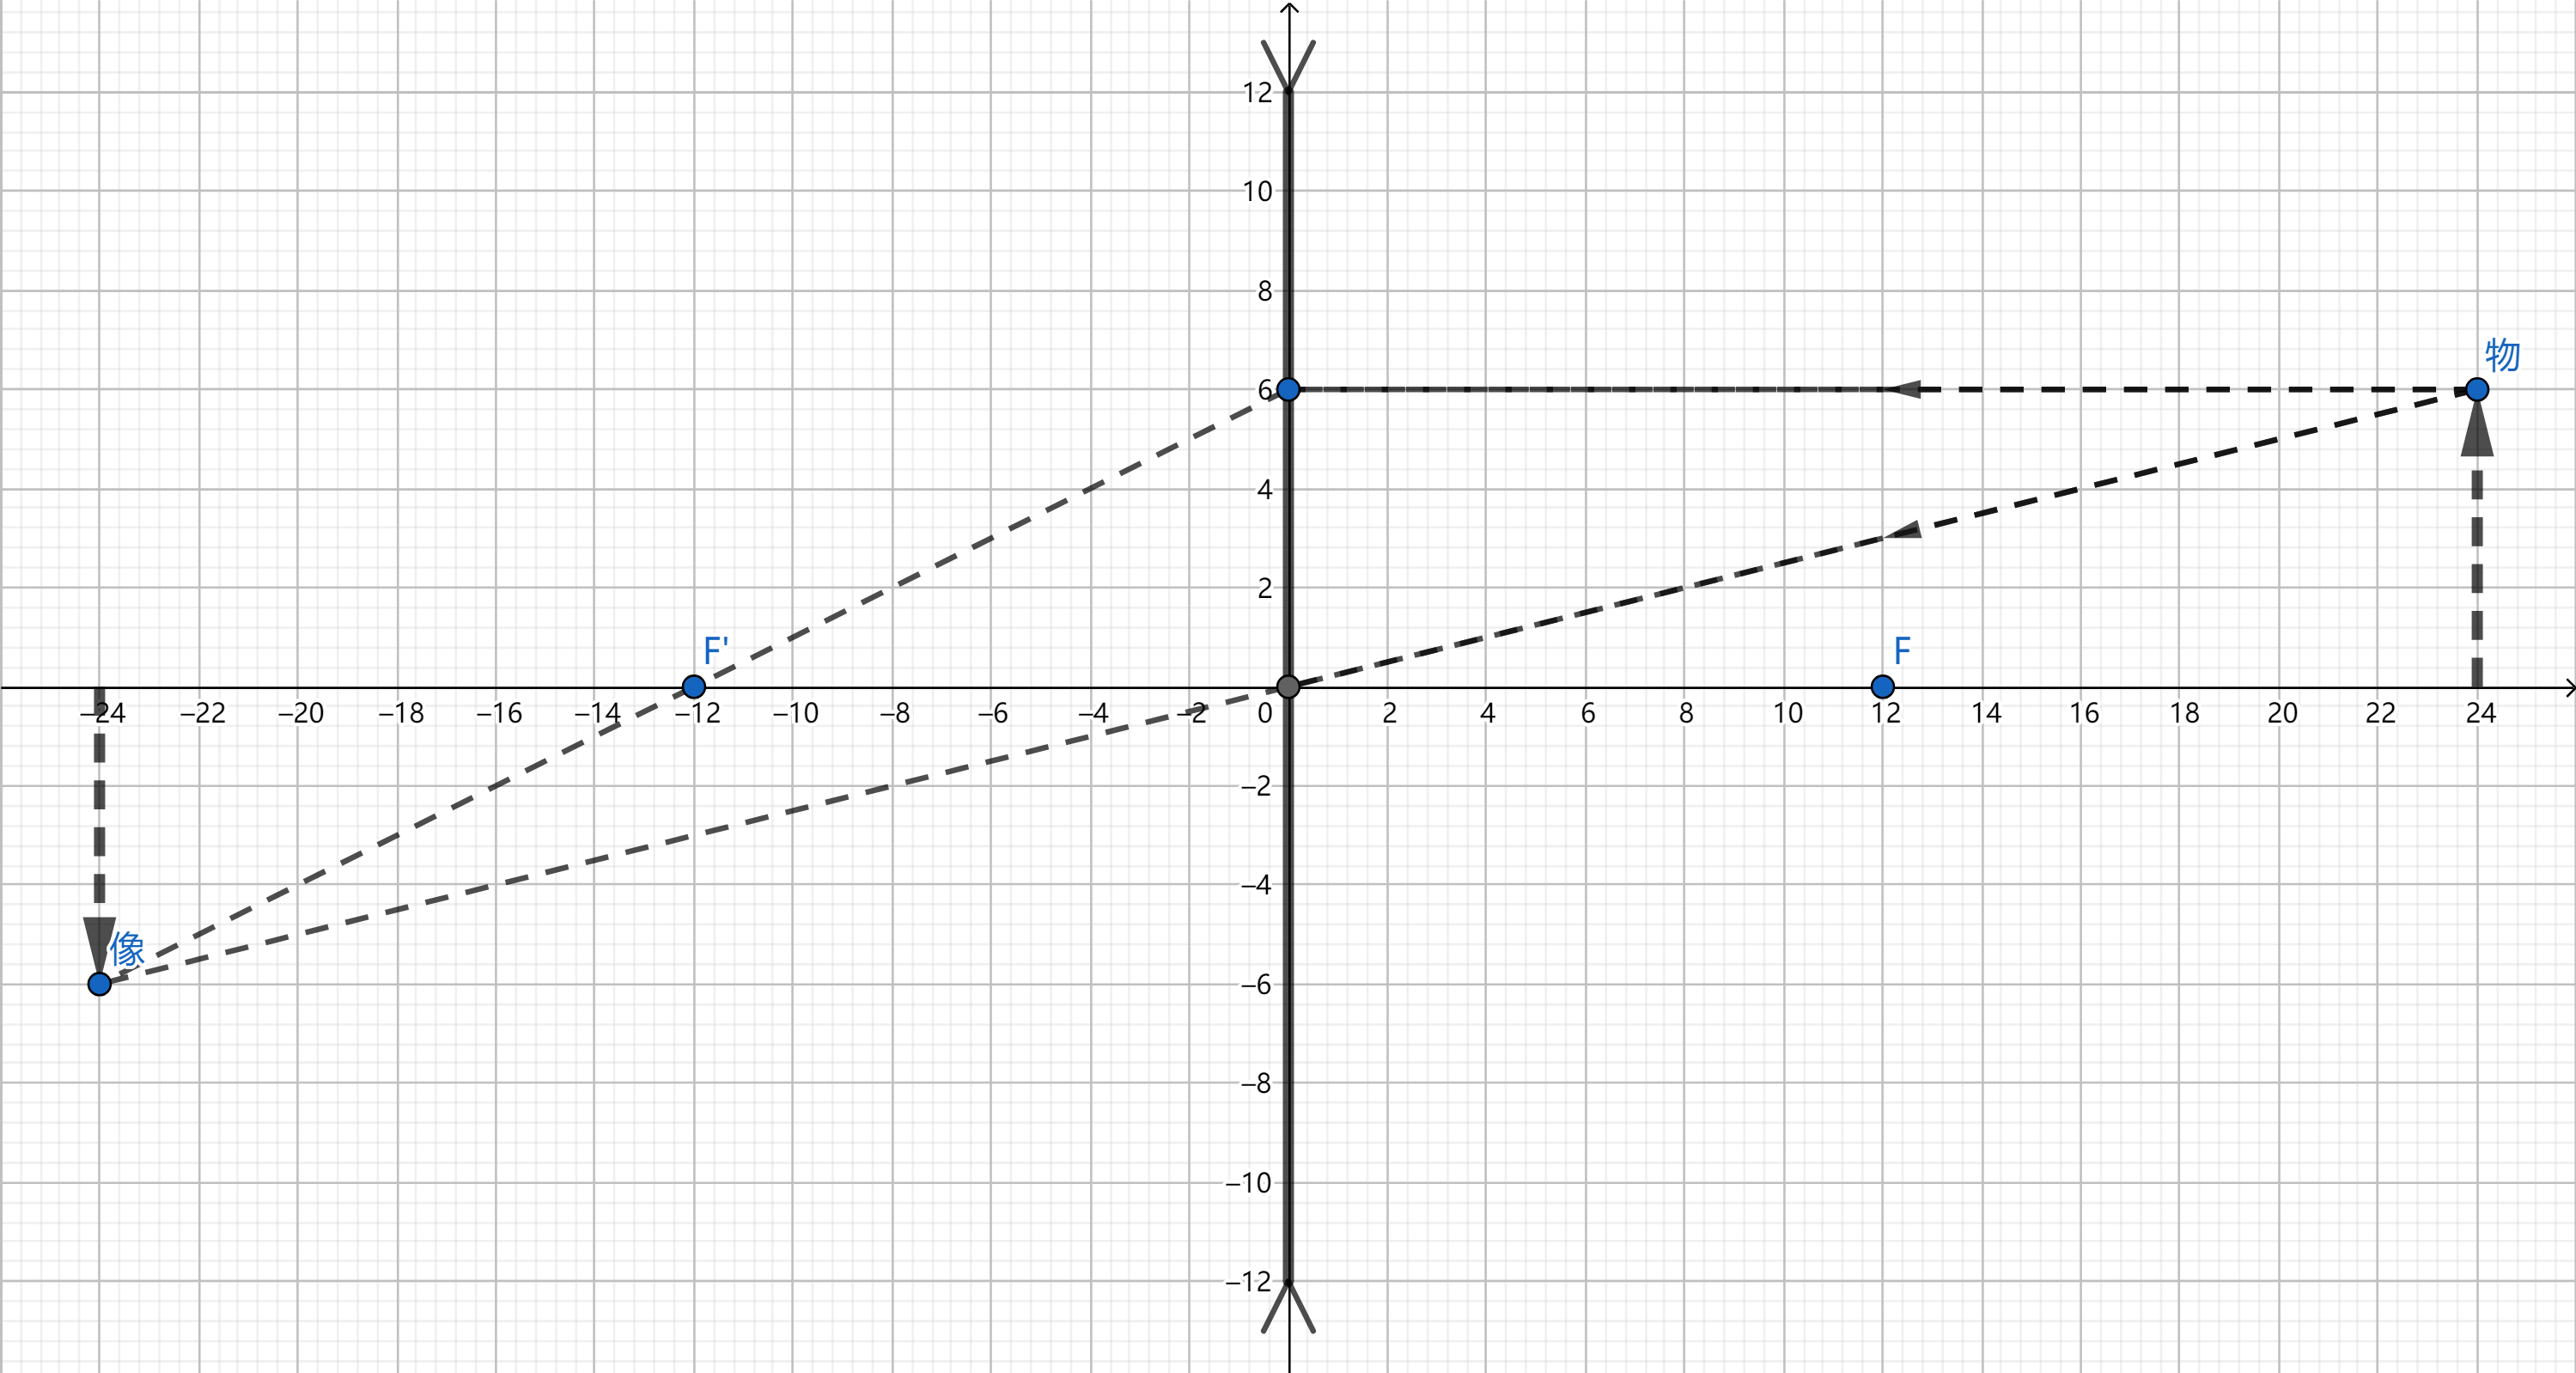
\includegraphics[scale=.2]{OpticsHomework_2_2-19_1(tailored).png}
\caption{2-19题图1}\label{FigureofProblem2-19_1}
\end{figure}

当物距为$-12cm$时,相应光路图如图(\ref{FigureofProblem2-19_2})
\begin{figure}
\centering
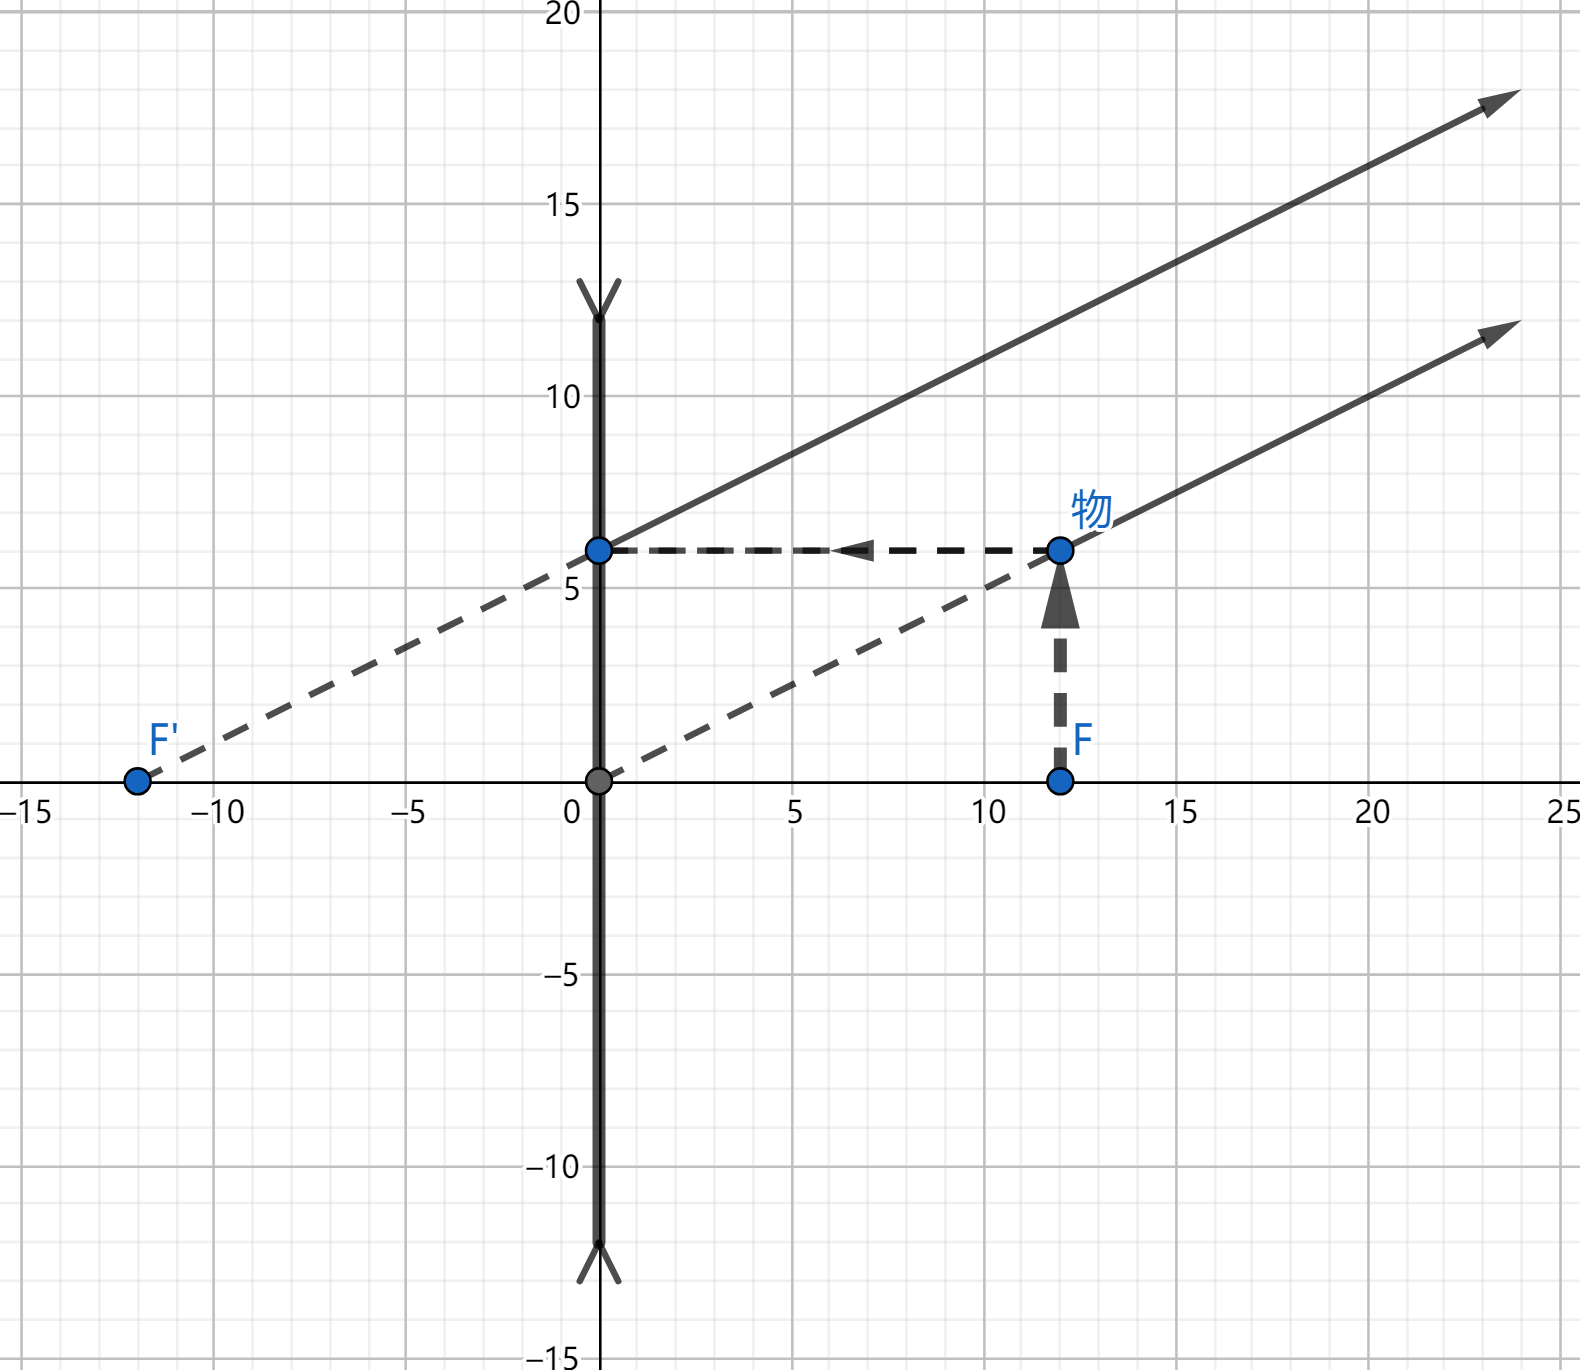
\includegraphics[scale=.2]{OpticsHomework_2_2-19_2(tailored).png}
\caption{2-19题图2}\label{FigureofProblem2-19_2}
\end{figure}

当物距为$-6.0cm$时,相应光路图如图(\ref{FigureofProblem2-19_3})
\begin{figure}
\centering
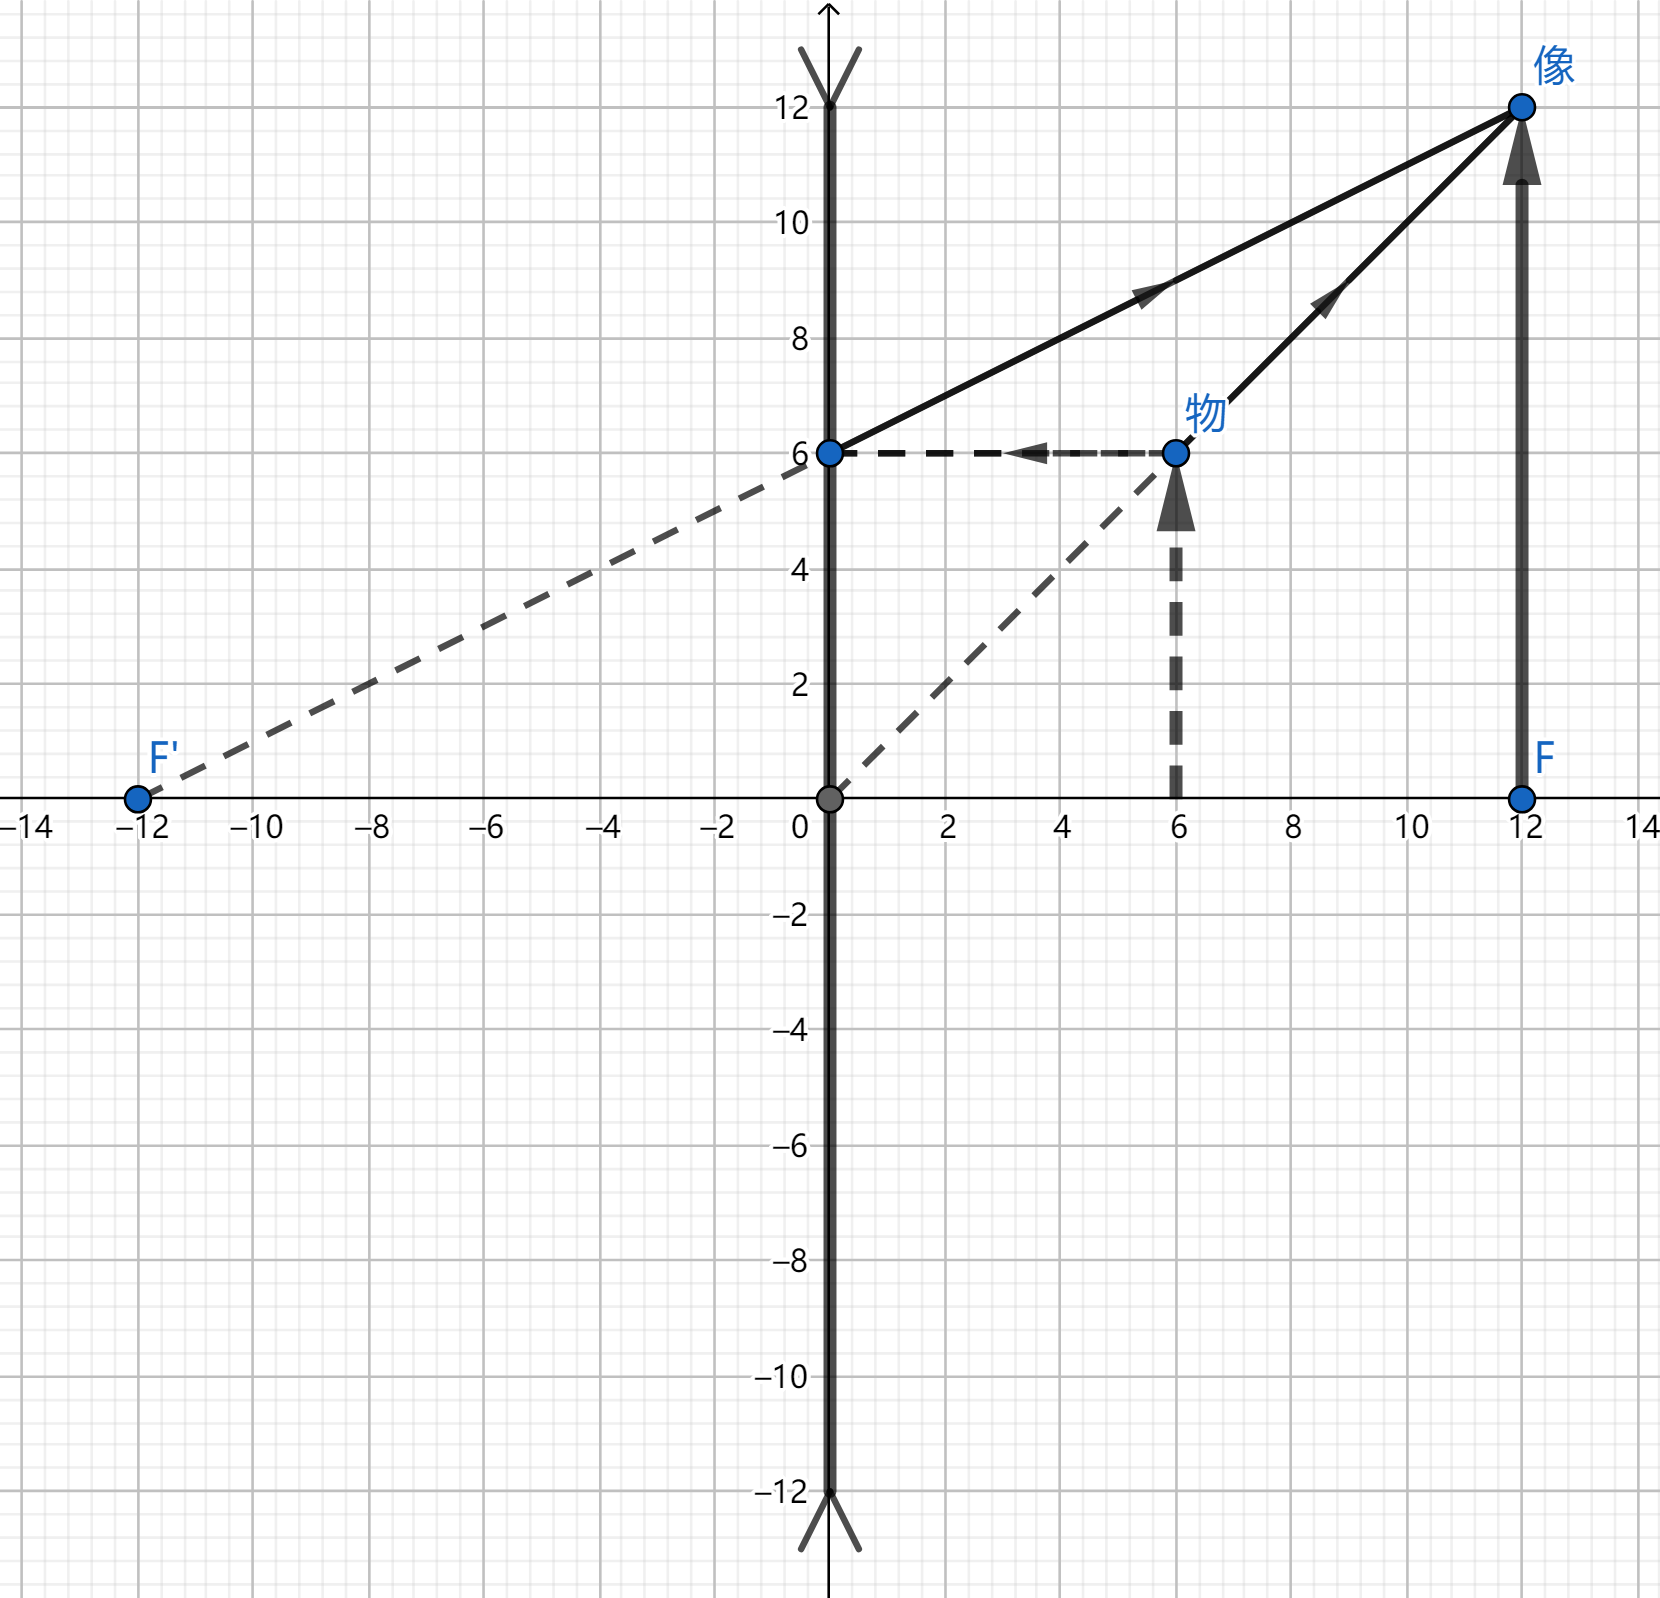
\includegraphics[scale=.2]{OpticsHomework_2_2-19_3(tailored).png}
\caption{2-19题图3}\label{FigureofProblem2-19_3}
\end{figure}

当物距为$6.0cm$时,相应光路图如图(\ref{FigureofProblem2-19_4})
\begin{figure}
\centering
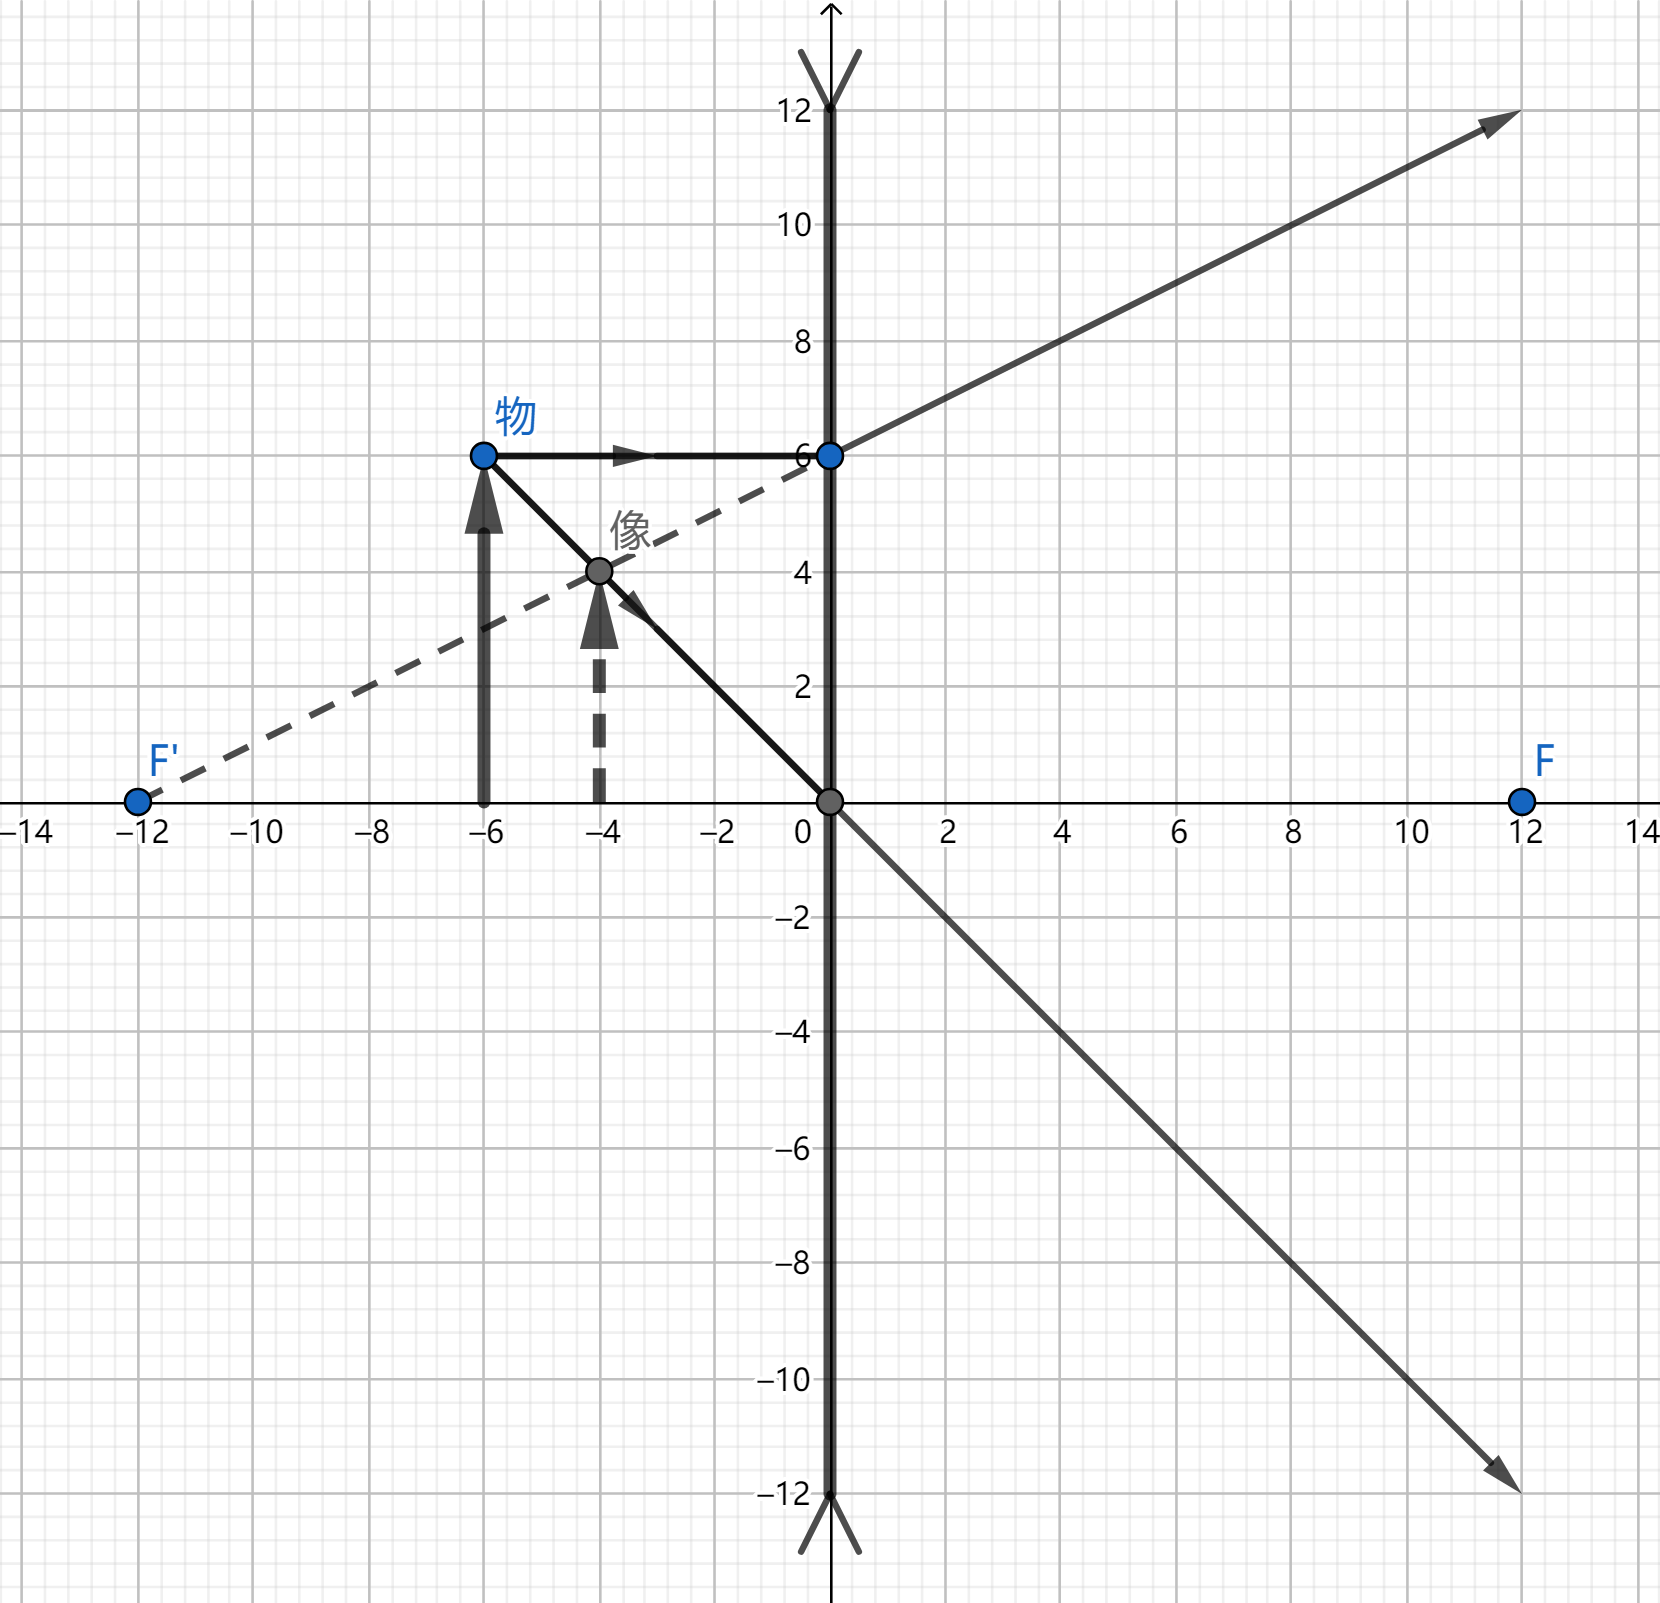
\includegraphics[scale=.2]{OpticsHomework_2_2-19_4(tailored).png}
\caption{2-19题图4}\label{FigureofProblem2-19_4}
\end{figure}

当物距为$12cm$时,相应光路图如图(\ref{FigureofProblem2-19_5})
\begin{figure}
\centering
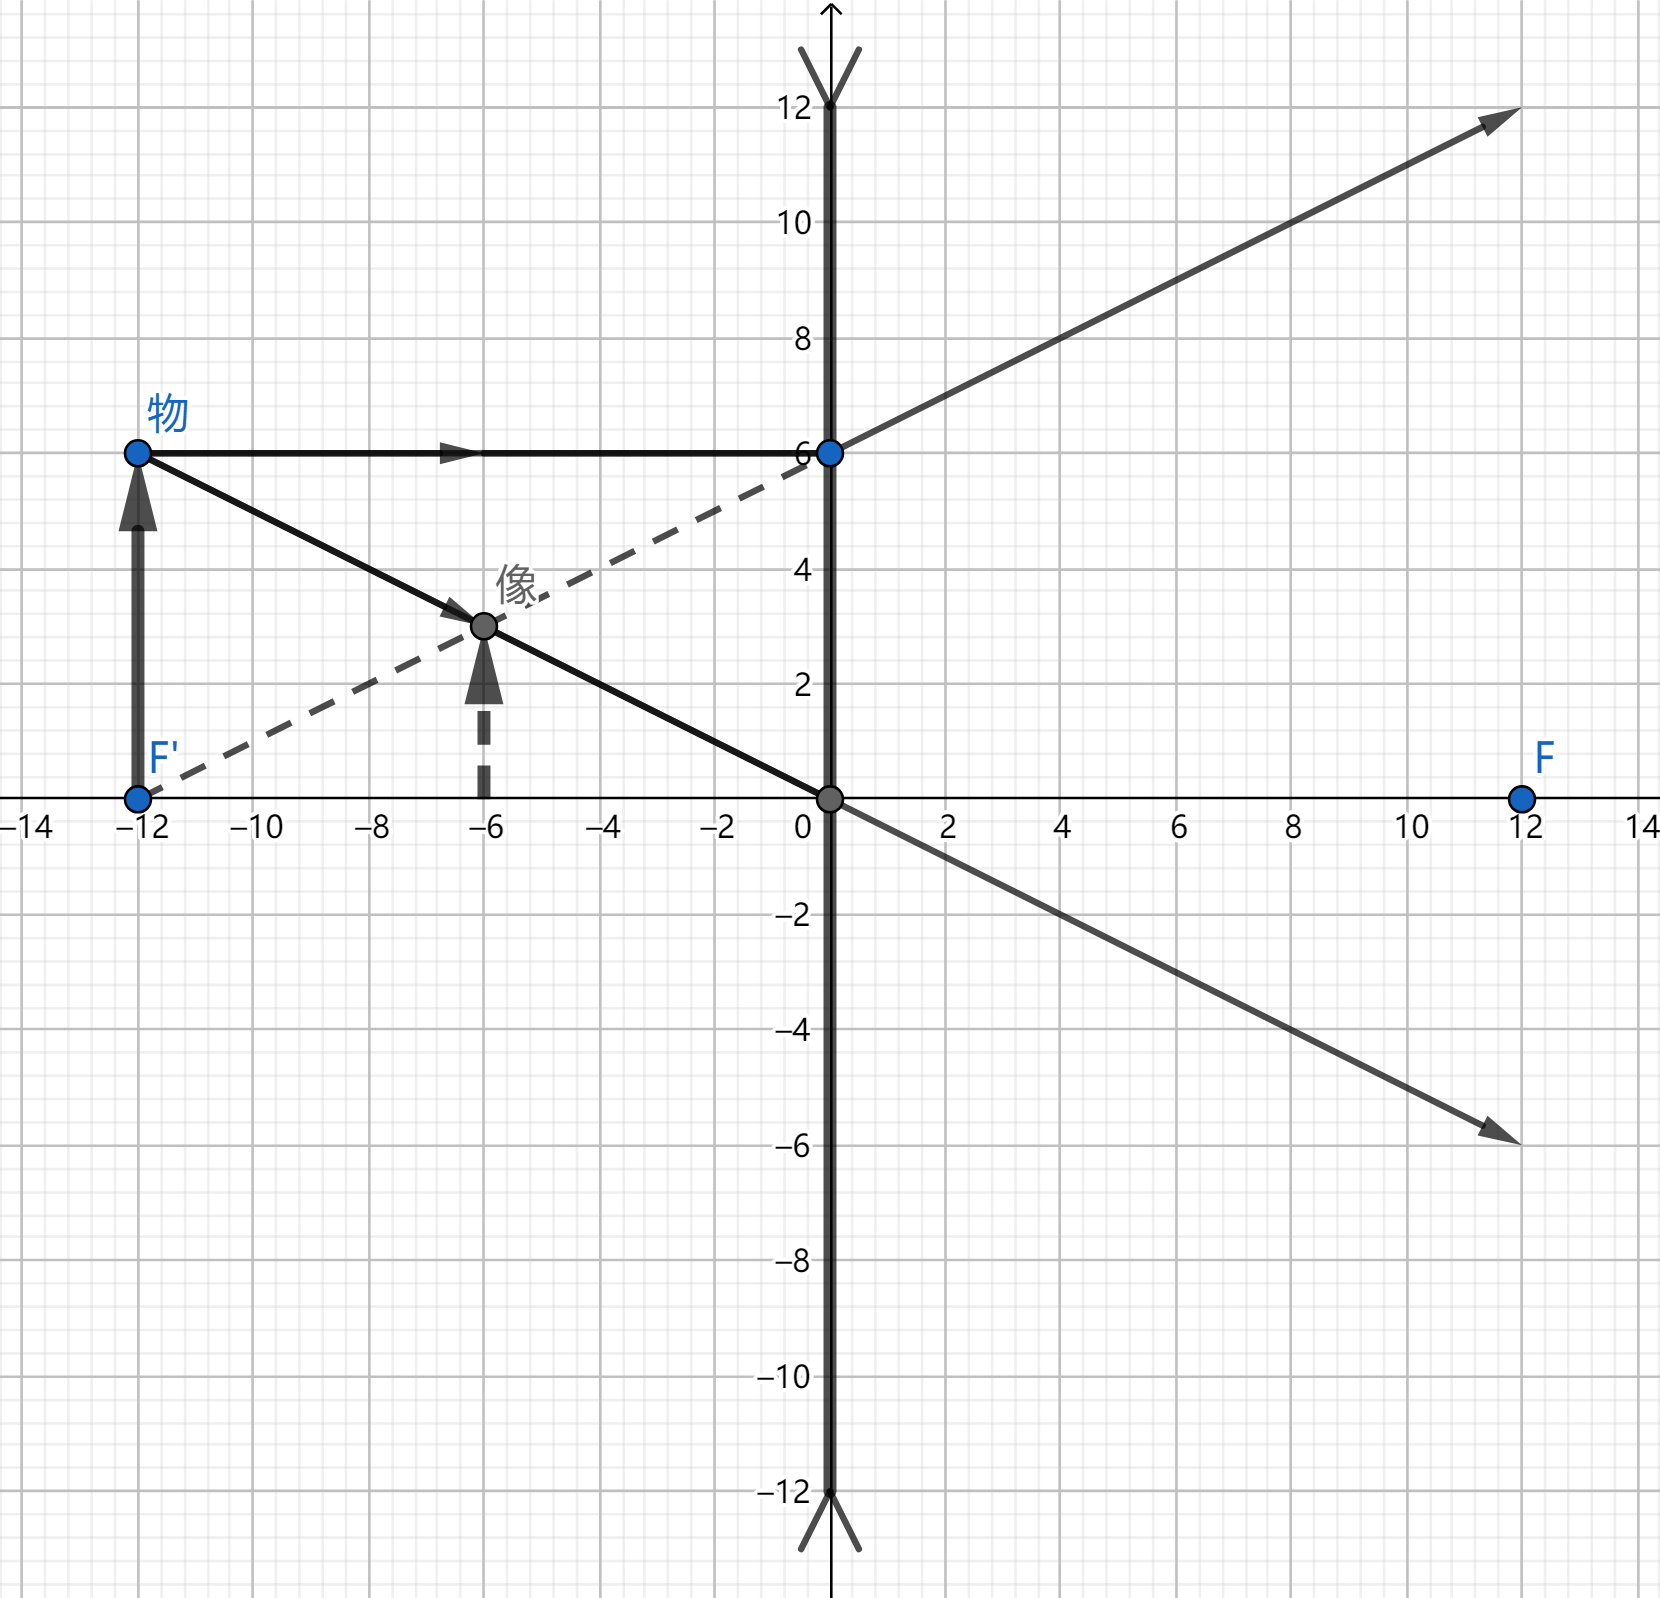
\includegraphics[scale=.2]{OpticsHomework_2_2-19_5(tailored).png}
\caption{2-19题图5}\label{FigureofProblem2-19_5}
\end{figure}

当物距为$24cm$时,相应光路图如图(\ref{FigureofProblem2-19_6})
\begin{figure}
\centering
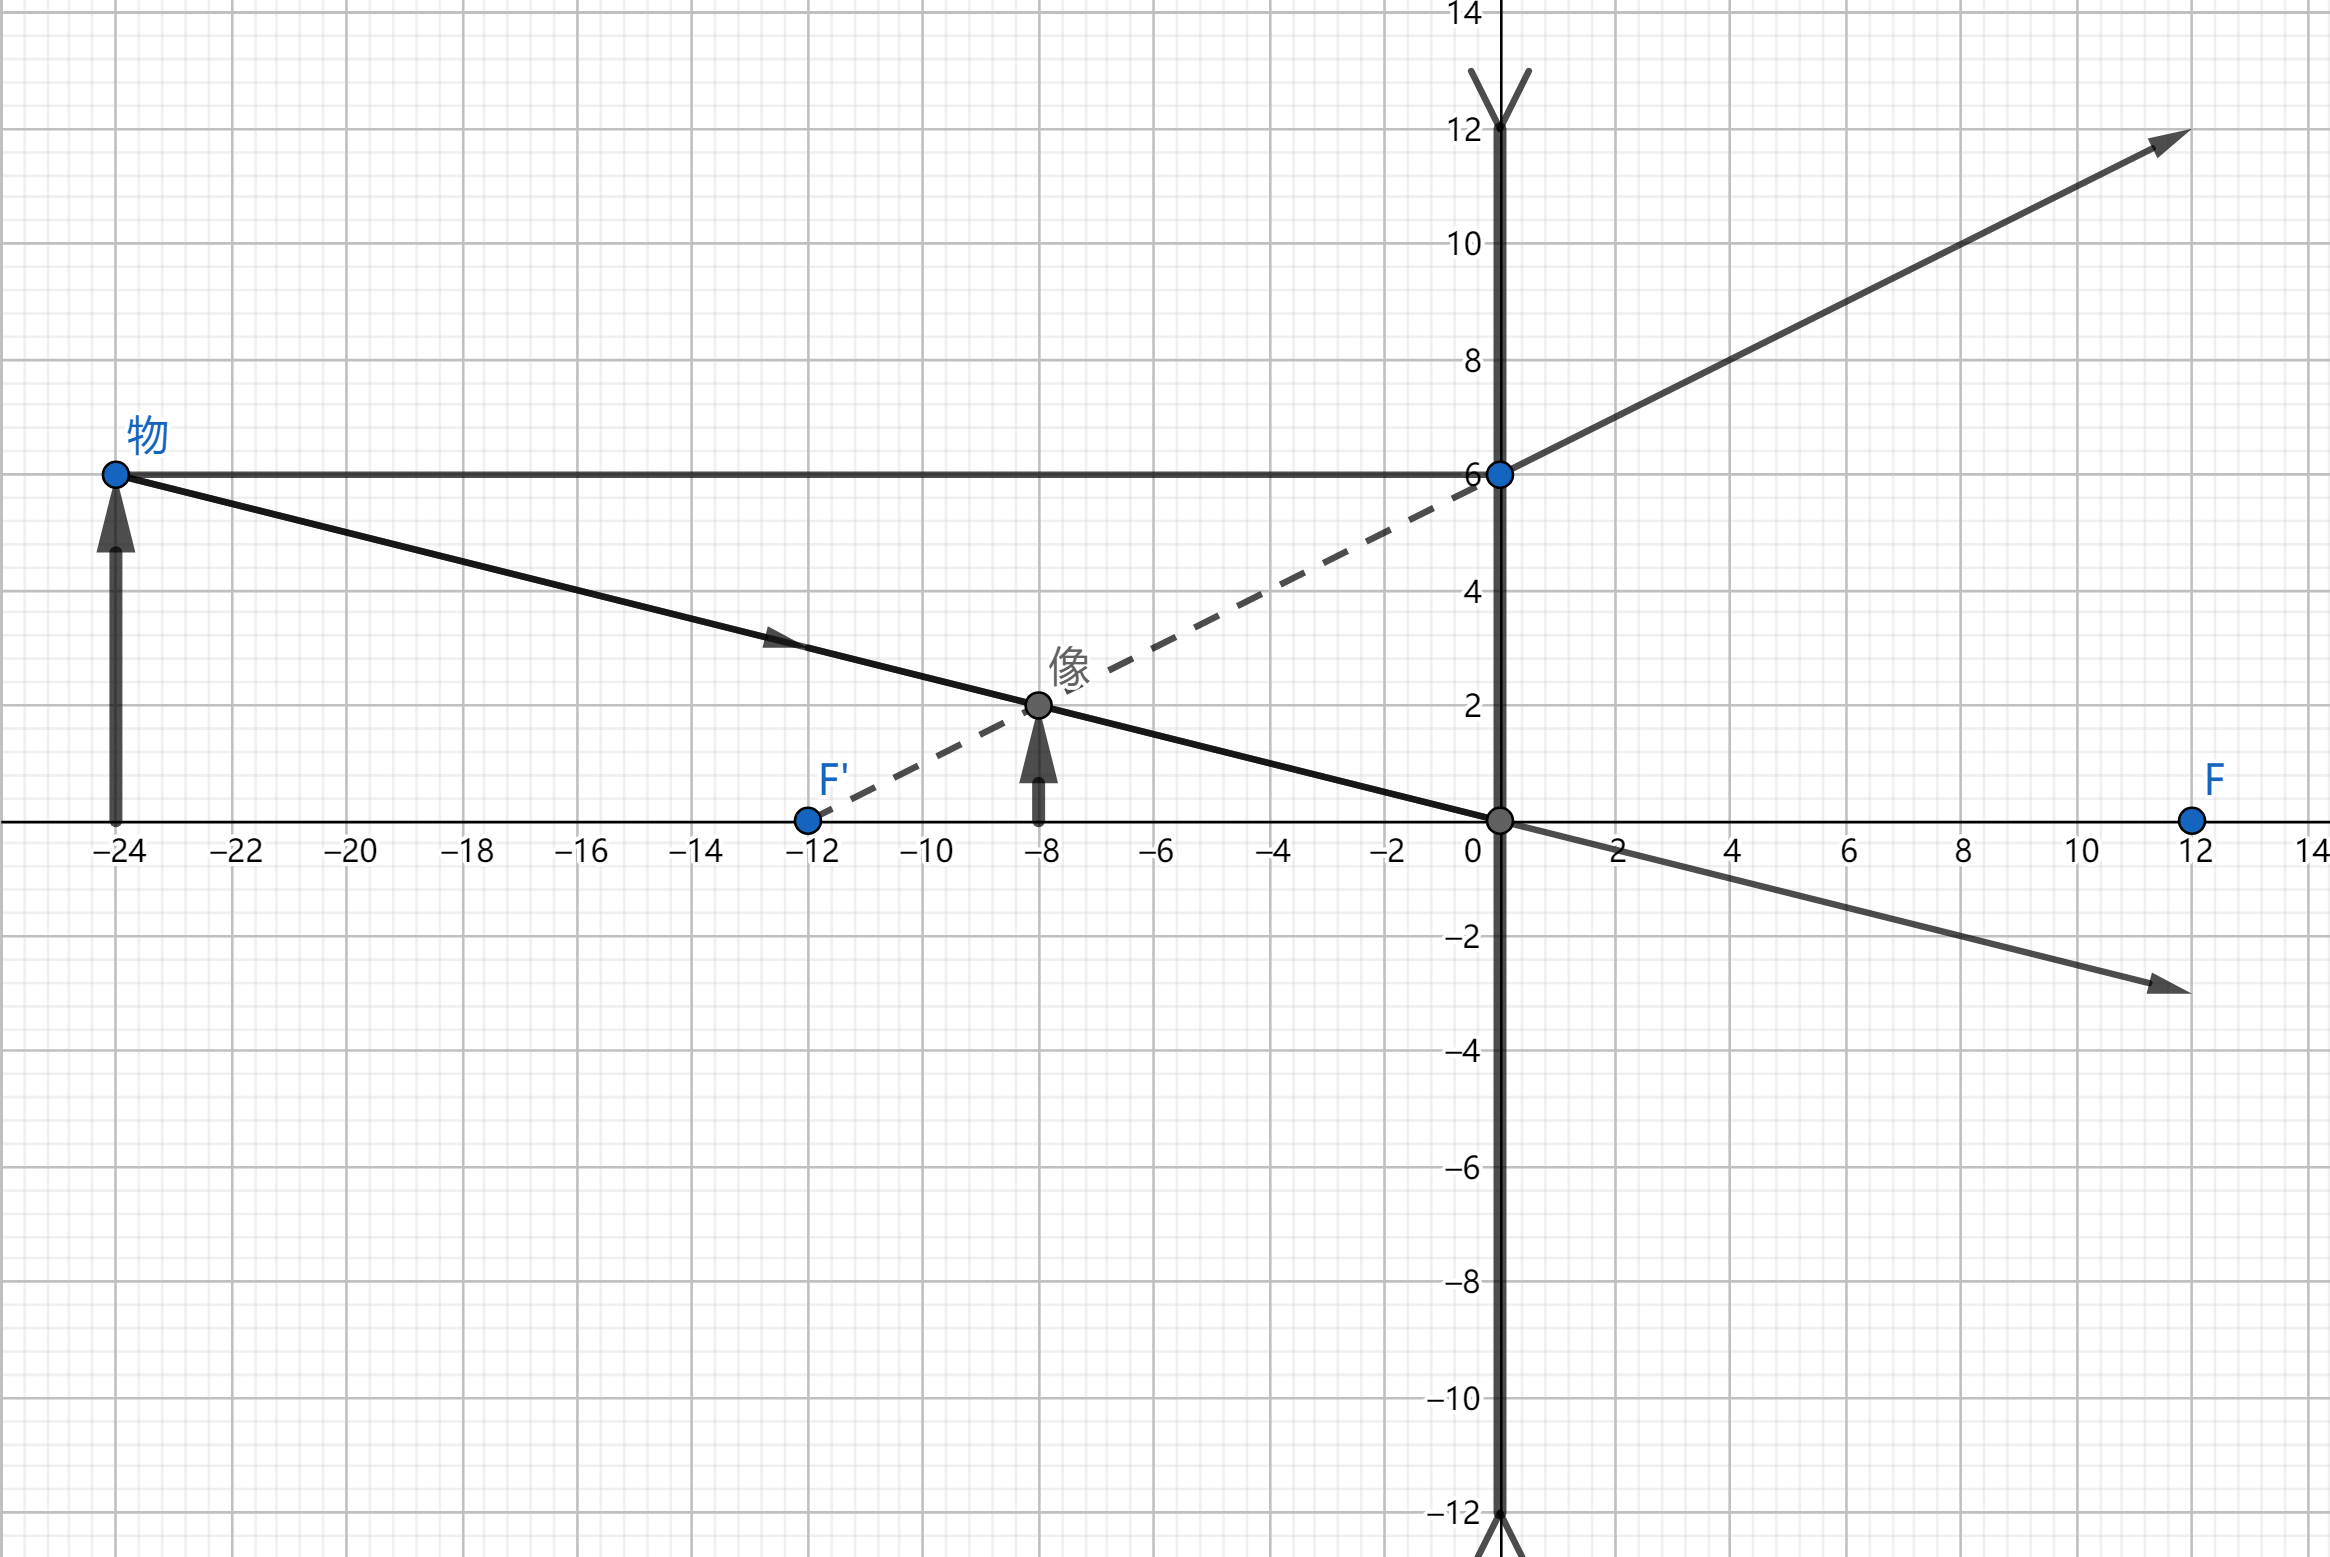
\includegraphics[scale=.18]{OpticsHomework_2_2-19_6(tailored).png}\\
\caption{2-19题图6}\label{FigureofProblem2-19_6}
\end{figure}

当物距为$36cm$时,相应光路图如图(\ref{FigureofProblem2-19_7})
\begin{figure}
\centering
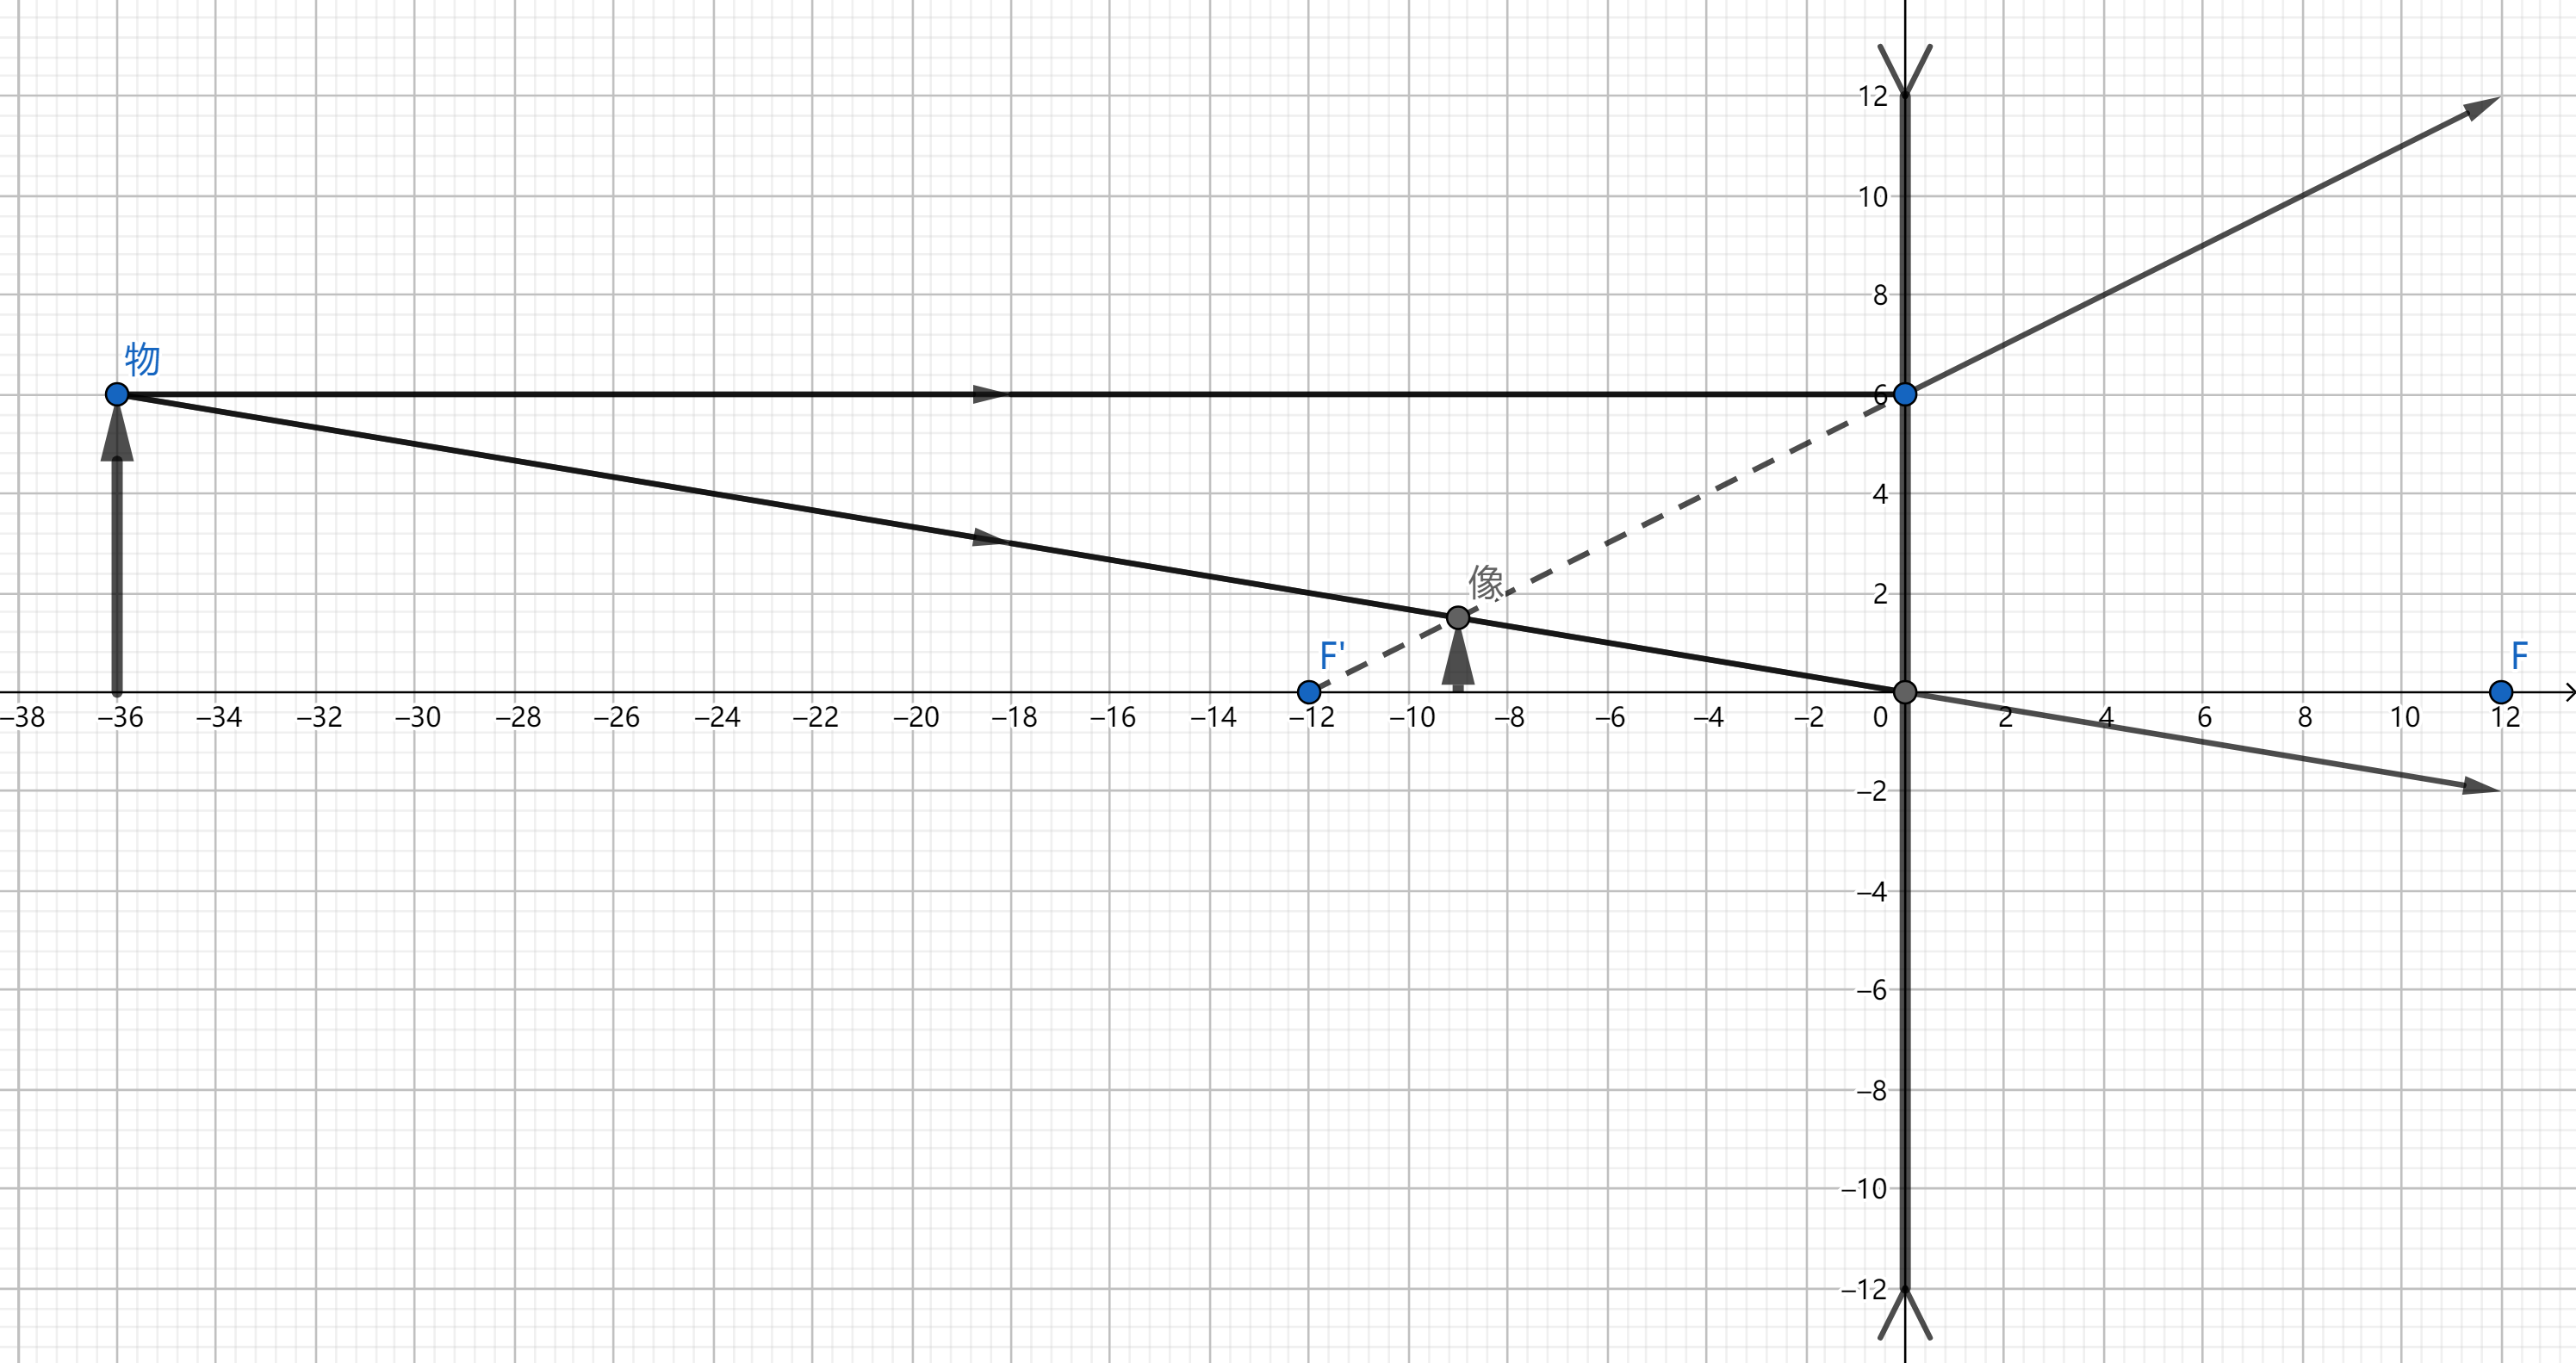
\includegraphics[scale=.15]{OpticsHomework_2_2-19_7(tailored).png}
\caption{2-19题图7}\label{FigureofProblem2-19_7}
\end{figure}

\section*{2-22}
\subsection*{(1)}解:
设凸透镜的焦距为$f$,物距为$s$,像距为$s'$,根据薄透镜物像距公式
\[
\frac{1}{s'} + \frac{1}{s} = \frac{1}{f}
\]
物、像距之间存在几何关系
\[
s + s' = 100(cm)
\]
两式联立得到关于物距的一元二次方程
\[
s^2 - 100s + 100f = 0
\]
根据题设透镜有两个位置可以使物成像在屏幕上且测得这两个位置之间的距离为$20.0cm$,故该一元二次方程存在两个差为$20.0(cm)$的实根,根据韦达定理
\begin{align*}
|s_1 - s_2| &= \sqrt{(s_1 + s_2)^2 - 4s_1s_2} = \sqrt{(-\frac{b}{a})^2 - 4ac} = \sqrt{(-\frac{-100}{1})^2 - 4\cdot1\cdot100f}\\
&= 20(cm)
\end{align*}
解得透镜的焦距为
\[
f = 24cm
\]
将其代入原一元二次方程中,解得物距的两根为
\[
s_1 = 40cm, s_2 = 60cm
\]
在这两种情况下,透镜的位置到幕的距离分别为$s'_1 = 60cm$和$s'_2 = 40cm$。
\subsection*{(2)}解:
两个像的横向放大率分别为
\[
V_1 = -\frac{s'_1}{s_1} = -\frac{3}{2}, V_2 = -\frac{s'_2}{s_2} = -\frac{2}{3}
\]
\section*{2-25}解:
光线第一次通过$L_1$折射成像,物像距公式为
\[
\frac{1}{s'_1} + \frac{1}{s_1} = \frac{1}{f_1}
\]
第一次折射物距为$s_1 = 10(cm)$,$L_1$焦距为$f_1 = 5(cm)$,解得第一次折射像距为
\[
s = 10(cm)
\]
横向放大率为
\[
V_1 = -\frac{s'_1}{s_1} = -1
\]
第二次折射通过$L_2$折射成像,物像距公式为
\[
\frac{1}{s'_2} + \frac{1}{s_2} = \frac{1}{f_2}
\]
第二次折射物距为$s_2 = 5 - s'_1 = -5(cm)$,$L_2$焦距为$f_2 = -10(cm)$,解得第二次折射像距为
\[
s'_2 = 10(cm)
\]
横向放大率为
\[
V_2 = -\frac{s'_2}{s_2} = 2
\]
故经此光学系统后所成的像的位置为$L_2$右侧$10cm$处,横向放大率为
\[
V = V_1V_2\\= -2
\]
(倒立、放大$2$倍的实像)。

作图(\ref{FigureofProblem2-25})(见下页)验证,与计算结果无异。
\begin{figure}
\centering
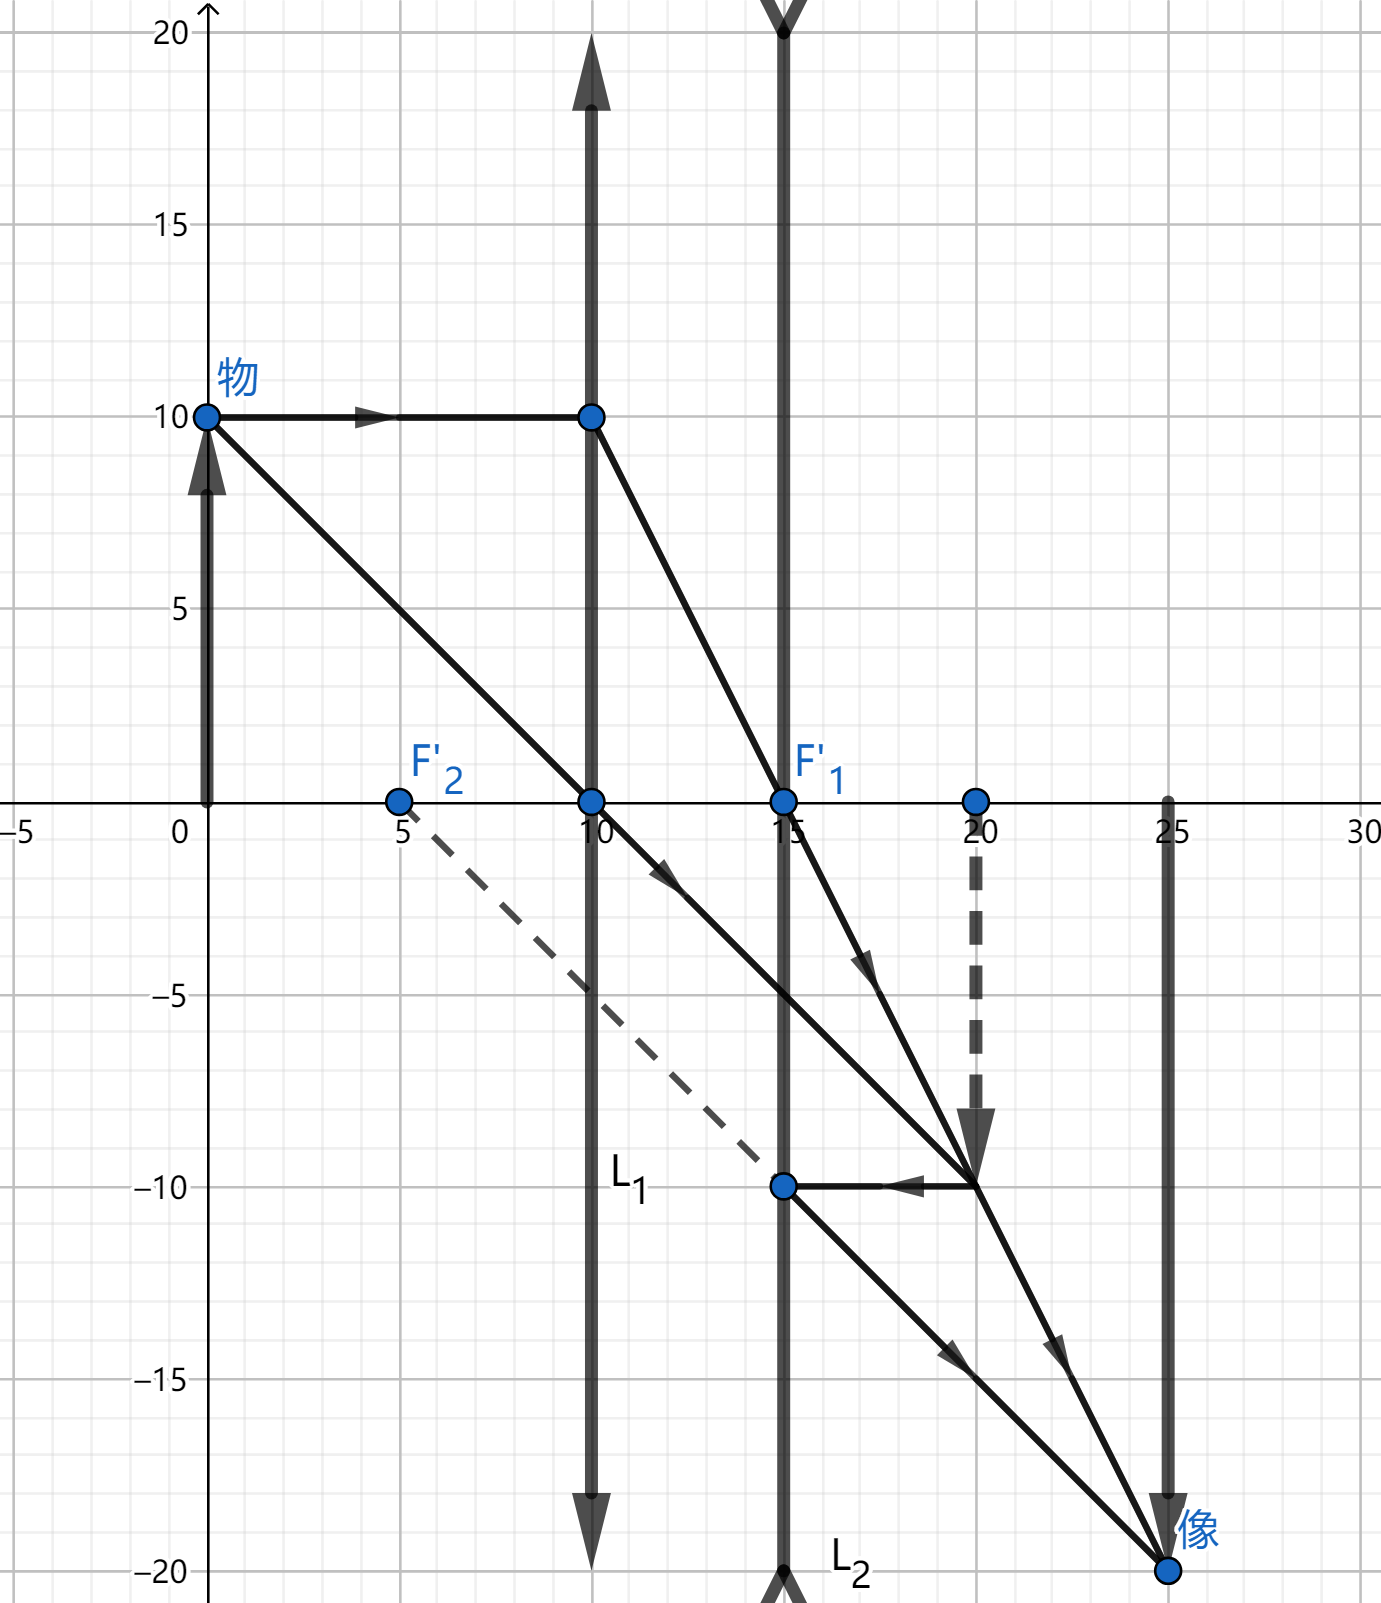
\includegraphics[scale=.3]{OpticsHomework_2_2-25(tailored).png}
\caption{2-25题图}\label{FigureofProblem2-25}
\end{figure}
\end{document}
